%!TEX root = project.tex

\chapter*{About This Project}
\paragraph{Analysis of This Project: }
%ADD references TO MERN STACK AND PYTHON HERE
This project was designed by me for the module Applied Project \& Dissertation with the purpose being
to complete an online banking system using a MERN(Mongo, Express, React \& Node) stack.
The project should allow user to login, view statements, takeout loans, perform transactions and
will show the user there monthly and yearly expenditures using graphs. The project will also be
secure and utilize user accounts using a mongo Database to ensure that the users account is secure.
\\*
\\*
The main purpose of this project is to utilize the MERN stack to provide a full and rich user
experience and to provide a secure, intuitive and polished online banking system.  The project
will also utilize Python scripts to perform statistical analysis on user expenditure and income
and will provide an estimate of how much money the user should have for the month based upon previous
monthly expenditure.
\\*
\\*
This project was designed to be a stand alone application where a user can perform all their
banking needs without any other software.  The user should be find the UI intuitive and the
features helpful.
\\*
\\*
This project will link many disparate technologies together for the purpose of providing the user
with the features they need.  I plan to use this project to show the skills I have attained during
my course and to learn a new framework(React). I also plan to improve and cultivate my skills
using new technologies such as various Python libraries and React. This project is stored on a GitHub
repository the link to which can be found in the appendix.
\paragraph{Authors: }
My name is \textbf{Ultan Kearns}, I am a fourth year student at GMIT. I have never used
React or \LaTeX\  before but I plan to learn a lot about these technologies during the course of this project.


\chapter{Introduction}
%Make sure you use references
\section {Why A MERN stack?}
\begin{center}

\includegraphics[width=\textwidth]{img/mern.jpeg}
\end{center}
There are many reasons why I have chosen to use a MERN stack for this
application the main one is because it provides a framework for a full stack
application.
MERN stands for \textbf{Mongo - For the database backend(Hosted on Mlab, all user info is stored here),
Express - A web application framework
host a server in a relatively short time compared to other methods
, ReactJS for asynchronous JS \& Node - For the server and also includes a package manager to install a variety of packages to provide certain functionalities.}
\cite{MERN}
\\
\subsection{Mongo}
As you have read above the MERN stack is very powerful in creating a full-stack
application when used correctly.  The reason I chose the database Mongo is because
it offers an open source alternative to MySQL and other proprietary databases
\cite{Mongo}
and many companies seem to be migrating to it because it is open source and in
some cases may offer better performance than other databases.
\begin{center}
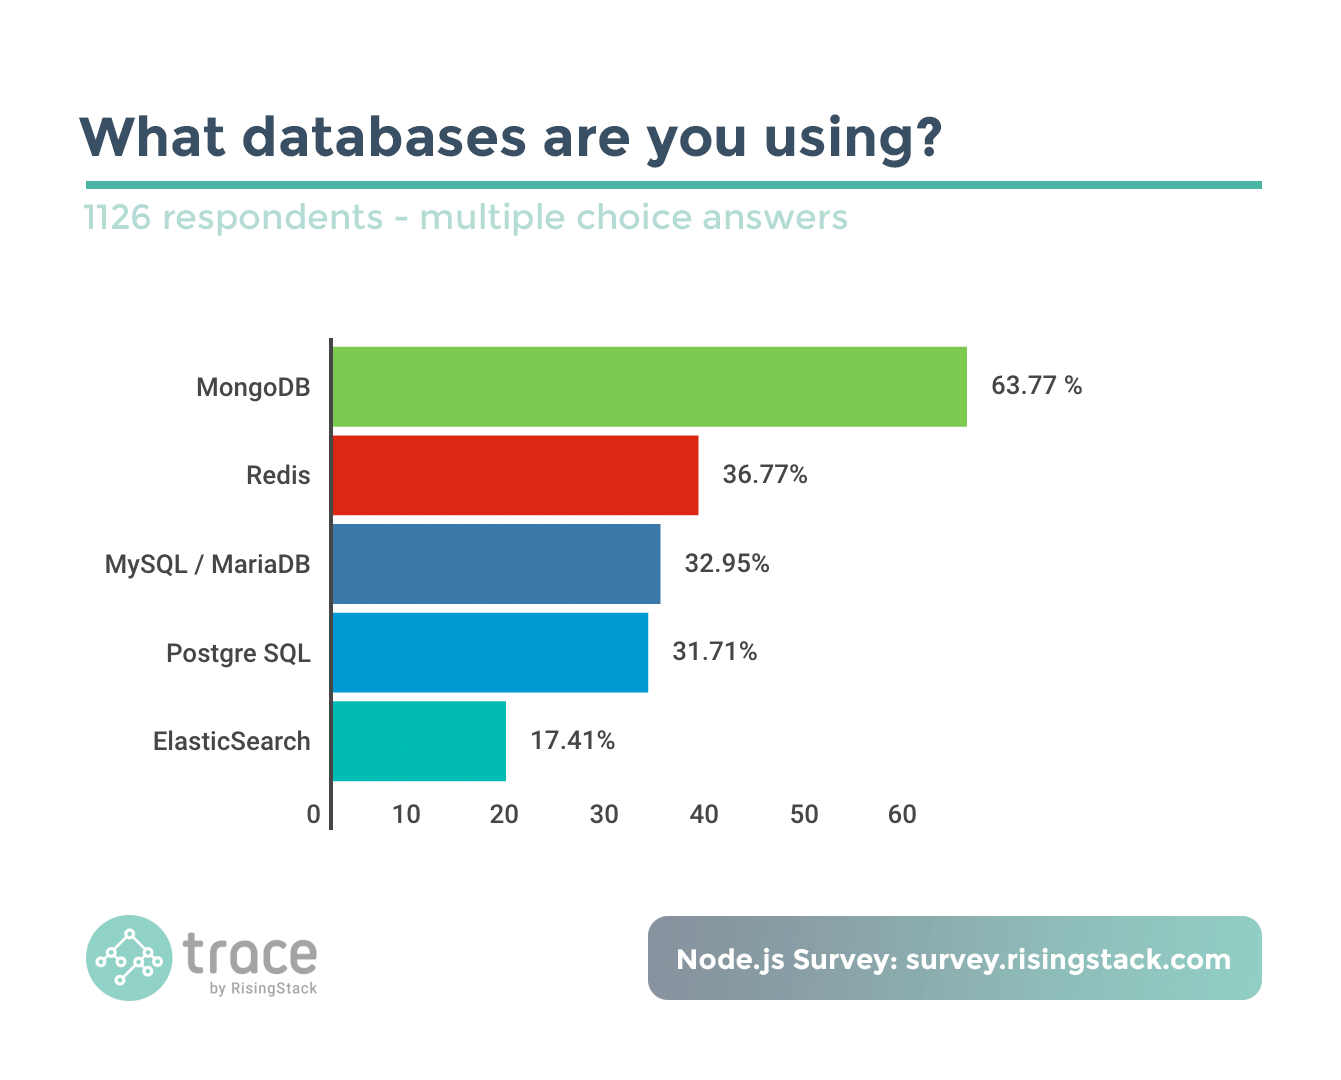
\includegraphics[width=\textwidth]{img/mongostat.png}
\end{center}
\cite{Survey}
Mongo is easy to learn as it stores it's data in JSON format and is schemaless, that is the user
defines their own schemas. I have also used it for 2 other projects in Angular and find it an
easy database to use in relation to projects.
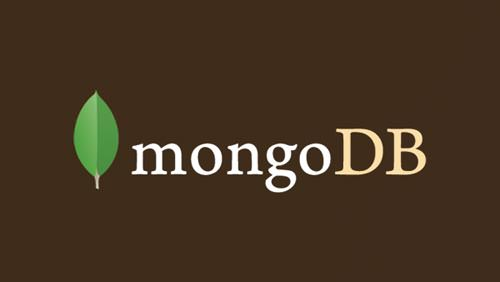
\includegraphics[width=\textwidth,height=4.5cm]{img/mongo.jpg} \cite{MongoImage}
\\
\subsection{Express}
I chose to use Express because it is a very useful framework when creating a server.
It is very helpful when pulling data from the server and displaying it to the client
it is also very scalable and offers good security when used properly.  It is also very
easy to setup and can be connected to the MLab database in minutes upon starting the
project.  I have also used this server before and have a bit of experience with it and
found it very helpful in the projects I used it for which were a messaging forum and an
E-commerce application both using MEAN(Mongo,Express,Angular \& Node) stacks.
\\
\includegraphics[width=\textwidth,height=4cm]{img/Express.png} \cite{ExpressImage}
\\
\subsection{React}
I also chose this project because I have zero experience in ReactJS and since
it's such an up and coming framework I decided on it for this project. It also
offers many features and libraries which are desirable when programming a user
interface to ensure the user finds the application intuitive and easy to use.
ReactJS also utilizes modular programming for components which makes designing
web applications far easier than just using HTML, CSS \& Javascript. React is
also very fast at rendering pages so that the user will not experience a major
delay in accessing information.
\\

\includegraphics[width=\textwidth,height=4cm]{img/react.png} \cite{ReactImage}
\\
\subsection{Node JS}
The reason I chose Node JS was because it offers a great package manager which can be
used to improve productivity on my part and also the applications security, UI,
UX and various other aspects of the application.  I debated using Yarn for this
project but settled on Node because it was already installed on my laptop.  Node
is a very useful tool when developing full-stack applications and was very helpful
in installing tools and libraries for react.  Node is also very good for getting a server
up and running in a few minutes and handles HTTP requests very well.
\\

\includegraphics[width=\textwidth,height=4.5cm]{img/node.png} \cite{NodeImage}
\\
\section{Why a banking application?}
\subsection{Explanation of Why I Chose This Project}
A banking application is broad in scope and offers many questions to the developer
such as how can I optimize load times and how can I ensure user data is secure.
I think questions such as these offer the potential for growth in the areas of
design and problem solving - which are two of the most major skills a software
developer can possess. I feel that an application such as a multi-user banking
system can be beneficial to my career and help to improve my skills as a developer.
Banking applications also have the potential to offer a wide array of features and
are ubiquitous in the real world, think major banks such as AIB \& Bank of Ireland.
Banking systems also offer a broad range of problems such as security, design
and usability.
\\
\subsection{My Contention With Existing Online Banking Systems \& How I Plan To Improve Upon Them}
The current generation of online banking systems or at least the ones I have used
tend to have a variety of problems.  These problems are glaringly obvious to most
people and the main problems include but are not limited to: usability, appearance, lack of
personalization \& lack of information given to user.  I will how I plan to solve each of
these problems below:
\begin{itemize}
\item \textbf{Usability:} I aim to provide an intuitive and cutting-edge user
interface using the latest react libraries to provide the user with an easy to
understand banking application.  All features will be easily navigated to using
a navigation bar and I will aim to make features as obvious as possible to the user.
\item \textbf{Appearance:} The UI of the modern day online banking system tends
to be absolutely depressing.  I aim to reduce this by adding in a responsive UI
and to offer the user a vibrant online banking experience.
\item \textbf{Lack of personalization:} I aim to make this application very personal
to the user by adding in personalized expenditure charts and giving the user a
unique and inimitable banking experience.
\item \textbf{Lack of information:} Modern banking applications sometimes display
a lack of information given to the user.  I plan to solve this by offering the user
expenditure charts, reports and also by sending automated emails to them when
their account balance falls below a user specified number.
\end{itemize}
\section{Requirements}
Below I will include the requirements for this application and expand upon them.
\begin{itemize}
\item \textbf{Multiple Users:} This application must allow multiple users to
execute simultaneous banking and user sessions must be independent of each
other.
\item \textbf{Secure:} Database information must be encrypted
\item \textbf{Accurate:} All statments and user information must be accurate.
\item \textbf{Login/Logout} The user must be able to login and logout
\item \textbf{information}: The user must be able to view all information related
to them (eg: statments, withdrawl dates etc.)
\item \textbf{Graphs/Charts}: The banking app must display expenditures and
credit in graphs and charts generated from python scriptss
\item \textbf{Emails} The application must be able to email the user a forgot
password if they forgot their password and alos be able to email the user if
budget controls are turned on.
\item \textbf{Register} The user must be able to register new accounts using
an email and password also ensure that it cannot be an email that already exists.
\item \textbf{Delete account} The user must be able to terminate their account
and all information that exists about the user must be purged from the server.
\item \textbf{Change information} The user must be able to update all their personal
information in relation to their account except obviously banking statments and
balances.
\item \textbf{User sessions} The application must use cookies to maintain a
user session and ensure that the cookies do not last more than a specified timeframe
max of a day.
\end{itemize}
\section{Outline of chapters}
Below I will outline the chapters that my Dissertation is broken up into and
give a brief outline of each one.
\subsection{Context}
In Chapter 2 I will discuss the context of my project and how online banking applications
have affected the modern age and traditional banking.  I will research how
online banking came about and how it is useful for the consumer as well as the
bank.
\subsection{Methodology}
In Chapter 3 I will discuss the methodology I followed and how it affected my
project and productivity.  I will also discuss my how I planned to complete the
project and discuss the methodologies I utilized in completing this project. I
will discuss why I chose these methodologies and give the reader an insight into
how this application was developed.
\subsection{Technical Review}
In chapter 4 I will discuss the technical aspects of this project and discuss how
they impacted the development of this project and why they were implemented. I
will discuss the MERN stack in more detail and how it was utilized to create a
full-stack online banking application.
\subsection{System Design}
In Chapter 5 I will explain the architecture and design of this project. I will
use graphs and diagrams to explain how the application is designed and how it will
function when deployed.  I will also present some of the code I used and how it
is used to perform various functions of the banking application.
\subsection{System Evaluation}
In chapter 6 I will analyze the finished product. I will test the system and evaluate
if it is up to standard and meets all the requirements I have specified. I will
test if the scalability, security and the UI to ensure that the user is provided
with the features outlined in the requirements section.
\subsection{Conclusion}
In chapter 7 will briefly outline what I learned from this project and highlight all
my findings from previous sections. I will also discuss the impact the project
had on my skills as a software developer and how it helped me to grow as a developer.
I will also discuss what I would do differently if I had to do the project over again.
\section{Structure of Project}
The \href{https://github.com/Ultan-Kearns/AppliedProject}{github project} contains two branches feature and master
I use the feature branch to test all new code and ensure that it works properly before merging it with the master
branch.  The git repository contains two folders banking-app and dissertation, the banking app folder contains the
main project and the dissertation contains all materials relating to the dissertation. In addition to the two folders
I also have a sprints.md file which contains information about all my sprints as I decided to use the agile methodology during this project, I also have a usefulresources.md file which contains a list of useful resources which helped me throughout the course of this project.  The final file is the README.md this will contain a brief intro to the project as well as information on running the application.
\chapter{Context}
\section{Project Objectives}
\begin{itemize}
  \item To provide safe \& secure online banking
  \item To provide an intuitive UI that can be easily navigated by the user
  \item To provide user generated statistical analysis of expenditure
  \item To provide a multi-user server and banking service
  \item To provide a RESTful API to the banking service(client/server totally independent
  ,stateless environment, caching)
  \item To provide a scalable application
  \item To provide user with security using encryption for the mongo database
  \item To limit loadtimes of traditional online banking eg. 365 Online Banking and others
\end{itemize}
\section{Online Banking}
Online banking is very relevant in today's modern world, the ease of access which
the digital age allows us has led to a significant amount of banking being done
online.  Think of how many inconveniences have been shed away by the advent of online
banking, no longer do people have to wait in line for ages at the bank to take out loans
or to view their statements as all this can be done online or with the help of computers.
Every modern bank now has some form of website which allows their customers to do
all their daily tasks related to banking online.  In this chapter I will discuss the
advantages, disadvantages and overall affect of online banking.
\section{History of Online Banking}
\subsection{Definition of Online Banking}
The definition of online banking includes any form of electronic payment systems
that allows the customer or business entity to conduct financial transactions
via a financial institutions website or application.
\subsection{The Beginning}
The metamorphosis of the old brick and mortar banks to the click and mortar banks of
today all started as early as the 1980s \cite{HistoryBanking}. The earliest version
of the online prescence of banking took place in none other than New York City, New York,
USA.  Citibank, Chase Manhattan, Chemical Bank and manufacturers Hanover became the
first banks to introduce on online banking system in 1981.\cite{HistoryBanking}
Then in 1983 the Bank of Scotland became the first bank in the UK to offer an
internet banking service which was called Homelink to UK customers.People had to
use their phones and their televisions to manage their online banking as computers
where not as ubiquitous at this time \cite{HistoryBanking} It was not until 1994
that a bank in the USA called the Stanford Federal Credit Union began to offer online
banking services to all of its customers \cite{HistoryBanking}.In the year 2006 80\% of US banks had began to offer
some variation of online banking \cite{HistoryBanking}.
It was a slow process to move from the tried and true brick and mortar banking that the majority of the public
were,if not entirely satisfied with, were familiar with and accustomed to through decades of
useage. The move from brick and mortar to click and mortar was not all advantages, there were many issues
which had to be addressed such as ease of access, security and the education of the public about phishing scams
and various other crimes which can occur by storing information online.  Some banks offered advice to the elderly
and people who may not know so much about computers advice in an attempt to cut down on online banking crimes I have refereneced an example of one such site targeting the elderly to dispense such advice \cite{BOIElderly}
\section{Advantages of Online Banking}
\subsection{Convenience}
There are many advantages to online banking which I will discuss in this section
the most prominent of these advantages is convenience.  Bank customers no longer
have to drive or walk to the bank or to an ATM to check their balance and with online
payments customers will never have to withdraw money unnecessarily.  You can now
easily transfer money between accounts online and set up standing payments to pay
your bills which is a lifesaver for some people. You can also use your mobile to
view your balance and statements anywhere using mobile data and online banking applications,
this allows users to access their account from anywhere in the world depending on the
availability of reception.
\subsection{Speed}
The speed of which a bank customer can access their account information is now
determined by the speed of their internet.  Before the advent of online banking
you would have to wait in line at an ATM to see your statements or to withdraw
money to pay your bills, now that online banking has become virtually ubiquitous
in the modern world you no longer have to wait in lines to perform activities and
tasks relating to banking.
\subsection{Competition}
The rise of online banking means that banks are constantly trying to out do each
other in terms of their banking applications.  The customer now has much more choice
in choosing banks since the advent of online banking. The advent of online banking has
led to some banks maintaining only an online prescence.\cite{OnlineBanking}
\subsection{Creation of Jobs}
The switch from physical banking to digital banking has created numerous jobs
in the software industry especially in terms of cyber-security as banks increasingly
worry about security braches and hacks.  Any hacks that occur are viewed as the fault
of the bank and allows many customers to migrate to other banks, that is why many banks
spend a lot of money to secure data on their servers which creates jobs and stimulates
the economy.
\section{Disadvantages of Online Banking}
\subsection{Security}
Storing details in a digital environment is a lot less secure than storing them
in a non digital format.  This happens because the data is stored on a server
and if phishing scams getting a user's password are successful they could find that
their bank account has been drained of money.  There are many other forms of attacks
which could occur such as keylogging, network monitoring and on public networks
your data is far less secure.  Although banks have taken many counter measures
to prevent such attacks from occuring sometimes they slip through the cracks of
cyber-security analysts\cite{BankHacks}.  Most people find that a little less security is a fair
trade-off for the convenience online banking provides.
\subsection{Layoff of Bank Employees}
As the migration of banking from physical to digital takes place it leads to
a surplus of banking employees which are made redundant.  This occurs because
of the ease of access of online banking and this limits the need for more
tellers in many banks.
\subsection{Increased Crime}
As banks migrate there is an increase of cyber-criminals who try to gain access
to the banks.  According to one article 25\% of all malware hits financial services
\cite{ForbesBankHack}.  This increase of crime leads to an increased number of compromised
accounts on a banks server.
\section{The Overall Effect of Online Banking}
The overall effect of online banking has had a stunning impact on our world.
The availability of a bank 24/7 has provided countless benefits to both consumers
and businesses alike.  The advantages in my mind as in the minds of many others
far outweigh the disadvantages of online banking.
\chapter{Methodology}
\section{Overview of Methodology}
In this project I utilized the Agile methodology, I used Sprints to coordinate my work and after each sprint I performed
module testing and regression testing.  I also used Test Driven Development which involves writing tests and writing just
enough code to make them pass and then going back and refactoring the code.
\section{Agile}
%% need to add referencess
\subsection{What is Agile?}
Agile is a software development methodology which according to the agile manifesto website \cite{Agile} favours: "Individuals and interactions over processes and tools,
Working software over comprehensive documentation,
Customer collaboration over contract negotiation,
Responding to change over following a plan".  There are many variations of agile \cite{VariationsofAgile} such as Scrum, XP, Kanban and many more. All Agile methodologies follow the same principles outlined in the Agile Manifesto\cite{Agile} For the purposes of this project I'll be using Kanban.  All Agile methodologies stress
continuous improvement and incremental delivery.
\begin{center}
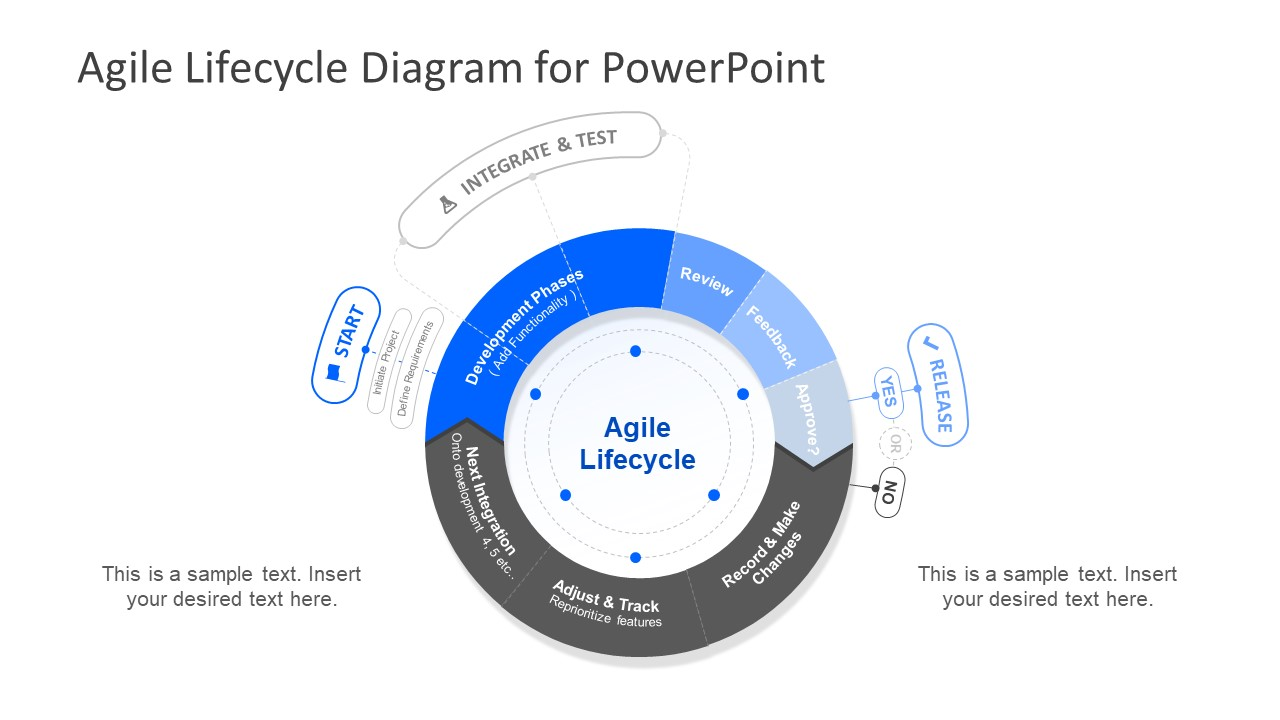
\includegraphics[width=\textwidth]{./img/agile.jpg}\cite{AgileImage}
\end{center}
\subsection{Why Kanban?}
Kanban \cite{Kanban} allows for a visualized workflow and was also easy to implement into the project. It allows for incremental development and a continuous improvement of features.  In contrast to waterfall, Agile methodologies also allow the developer to go back and improve upon features.  In summary Kanban offered me a visualized workflow and also allowed me to divide my sprints into daily or weekly tasks which I could complete in a relatively short time.
\begin{wrapfigure}{r}{0.1\textwidth}
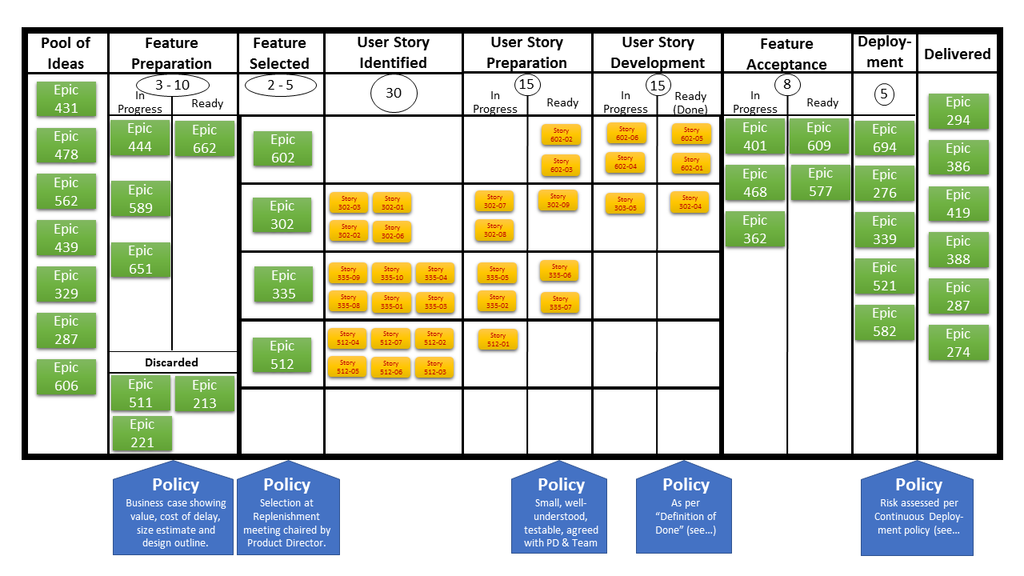
\includegraphics[width=3\linewidth]{img/kanban.png}
\caption{Image of Kanban board from wikipedia}
\label{fig:wrapfig}
\end{wrapfigure}
\subsection{How I Applied Agile To This Project}
During this project I used a Kanban board on Github \cite{KanbanBoard} to coordinate
my sprints(Backlog) and added the issues that needed to be finished to the Kanban board.   When an issue was added it was automatically moved to the "To Do" section of the Kanban board when it was in progress it was moved to the "in progress" section and finally when it was done I moved it to the "Done" section of the Kanban board.  The Kanban board helped create a visualized workflow which helped productivity as I could visualize which issues I would be working on that day and also I could coordinate
the Kanban board with my sprints to segregate work I needed to accomplish in a fixed
time-frame.
\section{Test Driven Development (TDD)}
\subsection{What Is Test Driven Development?}
Test Driven Development or TDD is a form of testing during development which focuses on writing the tests of a function before coding it and then writing enough code to make sure that it passes the test and then going back and refactoring it\cite{TDD}.
\begin{center}
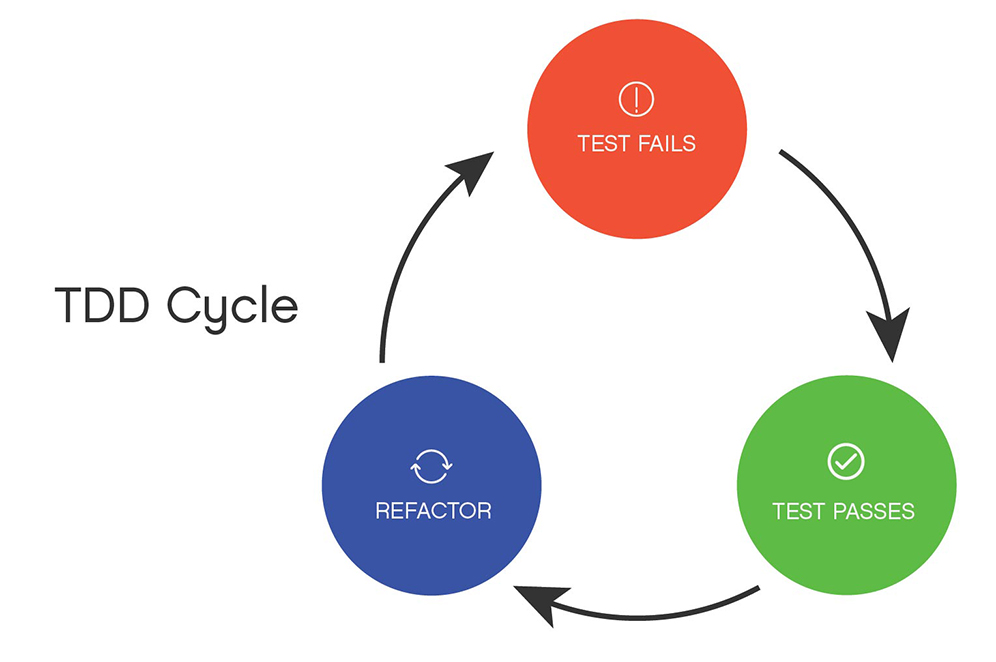
\includegraphics[width=\linewidth]{img/tdd.jpg}\cite{TDDImage}
\end{center}
\subsection{How I Applied Test Driven Development To This Project}
I wrote simple tests as I developed this code, for example for the statements section I wrote a test such as "Output only the statements of the user, output must be in form of location, cost, name, date" I then proceeded to write just enough code to make it pass and then went back and refactored it.
\section{Time Management}
\subsection{How I Handled Multiple Projects}
I was able to handle multiple projects at a time by defining sprints in my final year project and assigning myself daily tasks using the Kanban Board, sometimes I had issues in completing these daily tasks but I always tried to complete them in a timely and effective manner.  Sometimes I experienced scope-creep with a task where I had to add more features to the task to make the project viable.
\subsection{Issues I Faced With Time Management}
I faced some issues with time management as the workload was fairly heavy, I had to cut some projects short and leave out some features of various projects to ensure that all projects were completed to an acceptable level.
\section{Version Control}
\begin{wrapfigure}{r}{0.1\textwidth}
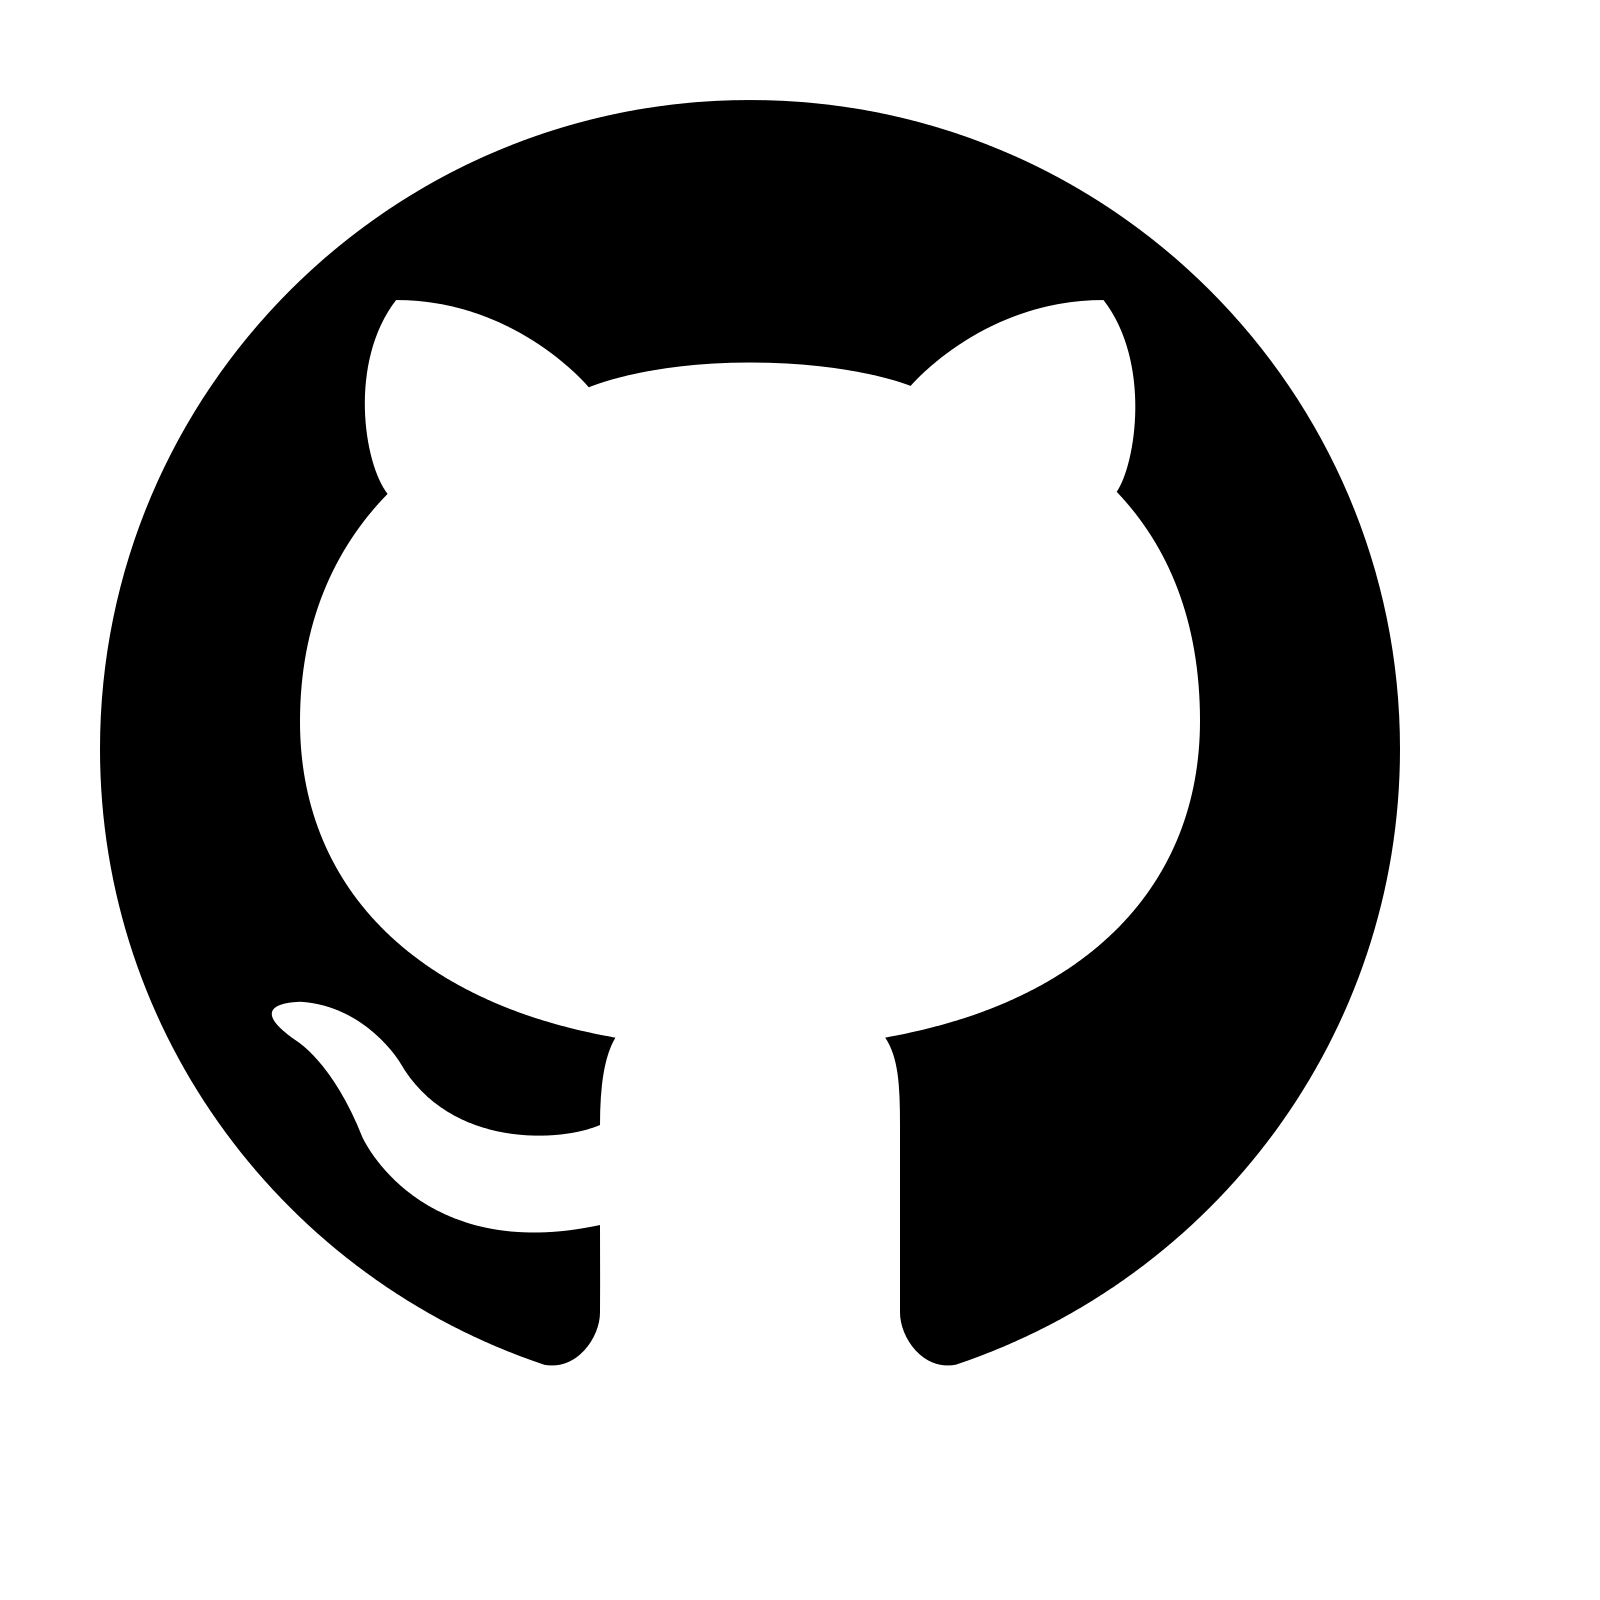
\includegraphics[width=3\linewidth]{img/github}
\caption{Github Logo from github.com}
\label{fig:wrapfig}
\end{wrapfigure}
I used GitHub to manage the versions of this application and to incrementally add code to my repository.
I also used GitHub for the Kanban board and to manage any issues that arose during the course of development.
\\
Github also allowed me to have multiple branches, one of which I used for all code that had been tested and was proven to work called Master and another where I implemented and tested desirable features, this branch I called Feature.  The compartmentalization of tested and untested code helped me a lot during the course of development as it allowed me to perform accurate regression tests and module tests which made
 debugging the application a lot easier.
\\
  Github also served as a backup of all my code in case of hard drive errors, hardware failures or various other issues that may arise.  Github also allowed me to revert back to previous versions of the project just in case I had made a mistake in the code and needed to revert back to a working version.  Github also served to provide me with a place were I could log any issues I had with the project and also allowed me to divide my sprints into daily or weekly tasks since the sprints were usually set over the course of a few days.
\chapter{Technology Review}
\section{Intro}
In this chapter I will explore the technologies I used in this project and why I used them.  I will also explain how the technologies were implemented and how they were utilized to ensure that the online banking application was fully functional.  I will also review the technologies I used in this project and show how each technology provided a desired functionality which would be paramount to achieving a fully fledged robust, secure and overall user-friendly baking system.
\section{MERN Stack}
The MERN stack is a technology which is used to make full-stack web applications.  Each component in a MERN stack has a specific function to allow for full-stack development.  The MERN stack is widely used in industry and is composed of the following components:
 \begin{itemize}
  \item MongoDB - For storing items in a database
  \item Express - Provides a web application framework
  \item React - A framework for making
  \item NodeJs - For server architecture and backend
\end{itemize}
\subsection{Mongo}

\subsection{Express}
Express is a Node.js web application framework which provides a myriad of desirable features for setting up a web sever.  Express helped me set-up a fully functional web application in a timely manner.  I also utilized Express to provide routing to multiple paths and to retrieve, delete, create \& update various information stored on my Mongo database.  I found Express very easy to setup and to use and the developers of Express provided comprehensive and very informative documentation on Express which can be found on their website\cite{ExpressDocs}
\\
 Express was able to return data I needed in JSON(JavaScript Object Notation) format and using the returned information I could then output the returned results to the user for purposes such as: to provide news \& to show the user their information.  I could also pass through parameters in the path and find information on a certain user or piece of data, this was very important for features such as logging the user in to the system as I had to compare the username and password and ensure both were correct.
 \\
 In conclusion Express provided a thin layer over Node.js to provide the application with features such as routing and also allows the developer to have a server up and running in minutes.  Express provided a lot of functionality to the banking application and also allowed me to create, read, update \& delete data, all of these are required for a fully fledged banking application in the 21st century.
\subsection{React}
\subsection{Node}
\section{RESTful API}
\section{Security}
\subsection{OpenSSL}
\subsection{SHA256}
\section{MLAB}
\section{Languages}
\subsection{Javascript}
\subsection{HTML(Hyper-Text Markup Language)}
\subsection{CSS(Cascading Style Sheets)}

\chapter{System Design}
As many pages as needed.
\begin{itemize}
\item Architecture, UML etc. An overview of the different components of the system. Diagrams etc… Screen shots etc.
\end{itemize}

\begin{table}[h]
  \centering
  \begin{tabular}{x{2cm}p{3cm}}
    \toprule \\
    Column 1 & Column 2 \\
    \midrule \\
    Rows 2.1 & Row 2.2 \\
    \bottomrule
  \end{tabular}
  \caption{A table.}
  \label{table:mytable}
\end{table}

\chapter{System Evaluation}
As many pages as needed.
\begin{itemize}
\item Prove that your software is robust. How? Testing etc.
\item Use performance benchmarks (space and time) if algorithmic.
\item Measure the outcomes / outputs of your system / software against the objectives from the Introduction.
\item Highlight any limitations or opportuni-ties in your approach or technologies used.
\end{itemize}

\chapter{Conclusion}
About three pages.
\begin{appendices}
\chapter{Preamble \& Intro}
\begin{itemize}
\item \href{https://github.com/Ultan-Kearns/AppliedProject}{Link to my github}
\end{itemize}
\end{appendices}
\bibliographystyle{ieeetr}
\bibliography{bibliography}
\end{document}
